\documentclass[12pt,fleqn]{article}\usepackage{../../common}
\begin{document}
Ders 1-20

Sona yaklasirken 4'uncu seviye bukulme denklemleri (4th order bending equations)
ve oge matrisleri konusunu biraz daha genisletmek istiyorum, hala sonlu ogeler
(FEM) dunyasindayiz, oge matrisleri FEM yaklasiminin ogeleri ve tam
matrisler.. Hatirlarsak makaskirisin her cubugu $A^T A$'nin bir parcasini
veriyordu, ve bu parcalar birlestirilerek $K$ olusturuluyordu. Bir cizitte her
kenar bir satira 1, -1 diye tekabul edecek sekilde bir matris ortaya
cikartabiliyordu.. Simdi oge matrislerinin FEM ile iliskisini yakindan gormek
istiyoruz. Bugunku dersin yarisi bu.

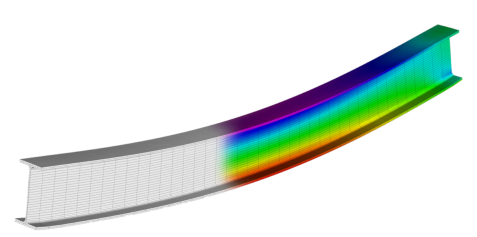
\includegraphics[width=10em]{compscieng_1_20_01.png}

Dersin diger yarisi 4'uncu derece diferansiyel denklemler. Simdiye kadar
gordugumuz tum diferansiyel denklemler ikinci derece idi, 4'uncu derece onemli
denklemler var mi diye merak edenler olabilir, evet var. Kiris bukulmesi
problemi bunlardan biri mesela, altta bu tur insaatlarda kullanilan turden bir
kiris goruyoruz, resim bir stres analizi programindan alinmis, mavi, yesil,
kirmizi renkler kiris uygulanan yukun etkilerini gosteriyor, kirmizi en fazla
stres olan yerler mesela, iste ustteki turden ciktilar 4'uncu derece bukulme
denklemini gerektiriyor.

Bu tur denklemler bizim $A^T C A$ altyapimiza uyuyor mu? Muhakkak oyle,
birazdan gorecegiz. 

Tek boyuta donus yapalim, analiz edilen cismi parcalara bolecegiz, ve her parca
bir ogeye tekabul ediyor olacak. Cisim bir buyuk cubuk, kiris olabilir..  Sonlu
farkliliklar (finite differences) ile size aralari esit olmayan izgara noktalari
versem ki alttaki resimde mesela $h$ ile $H$ birbirinden farkli olsa, bu FD ile
bizi bayagi ugrastirirdi, ikinci farkliliktaki -1, 2, -1 satiri yerine biraz
daha dengesiz degerler elde ederdik, bu izgaranin dengesizligi sebebiyle
olurdu. FD ile bu durumu ciddi tartmak gerekirdi, FEM ile sistem o dusunme isini
bizim icin hallediyor, dengesizlikler, oldugu yerlere sistemin yapisi
sayesinde dogal olarak cozuluyor. 

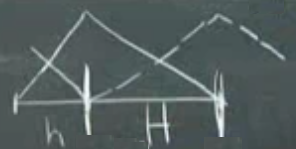
\includegraphics[width=10em]{compscieng_1_20_02.png}



















[devam edecek]

\end{document}
















